\documentclass[a4paper,10pt]{report} %,landscape
\usepackage[utf8x]{inputenc}
\usepackage{multirow}
\usepackage{graphicx}
%\usepackage[table]{xcolor}
\usepackage{lscape}
% Title Page
\title{Multi-Objective Divide-And-Evolve \\(MODAE$_{x}$)}
\author{}


\begin{document}
\maketitle
 
 
 \begin{landscape}
\begin{table}[ht!]
\caption{Algorithms comparaison according to Wilcoxon signed rank test with respect of the I$_{\varepsilon^+}^{1}$ metric. For each algorithm, either the algorithm located at a specific row significantly dominates the algorithm located at the specific colum ($\succ$ for a \textit{p}-value less or equal to 0.05), either it is significantly dominated (\textit{ p}-value up than 0.05), or there is no significant difference between both ($\equiv$) }
\label{ss}
\centering
\scriptsize
\begin{center}

\begin{tabular}{|l|l|c|c|c|c|c|}
   \hline
    \multirow{2}*{Instances}  &  \multirow{2}*{Algorithms}  &  \multirow{2}*{Average} &  \multicolumn{4}{c|}{ Algorithms}\\
    \cline{4-7}
	      &             & 	      		& $DAE-IBEA_{\varepsilon}$ &  $DAE-IBEA_{\textit{h}}$ &  $DAE-NSGAII$ & $DAE-SPEA2$  \\
   \hline
  \multirow{4}*{zeno$_{add}$}       & $DAE-IBEA_{\varepsilon}$    &  2.36e-01   &  --  		& 		$\equiv$       &  	$\prec$	&  	$\prec$		   \\
				
				    &  $DAE-IBEA_{\textit{h}}$	   &   1.91e-01
   & $\equiv$      	& 	--       & 	$\equiv$ 	&	$\equiv$      \\
				    &    $DAE-NSGAII$          &    1.77e-01     & $\succ$ (0.025)& 	$\equiv$ 	&	--		& $\equiv$   \\
				    &    $DAE-SPEA2$       & 1.74e-01     &  $\succ$(0.01)	&	$\equiv$ 	&	$\equiv$ 		 &  --  \\
  \hline
  \multirow{4}*{zeno$_{max}$}       &  $DAE-IBEA_{\varepsilon}$ &  2.19e-01  &-- &$\equiv$  & $\equiv$  & $  \succ $ (0.025)\\
	      &  $DAE-IBEA_{\textit{h}}$ 	    &        2.81e-01 &$\equiv$  &-- &$\equiv$  &  $  \succ $ (0.025)  \\
	      &  $DAE-NSGAII$	    &      1.95e-01   &$\equiv$  & $\equiv$  &-- & $  \succ $ (0.005)  \\
	      &  $DAE-SPEA2$		    &     4.54e-01    & $\prec$ &   $\prec$ &  $\prec$ & --   \\
   \hline
    \multirow{4}*{p01$_{add}$}   &    $DAE-IBEA_{\varepsilon}$   	    &   2.17e-001
      &    --  		& 		$\equiv$       &  	 $\prec$	&   	$\prec$	   \\
	      & $DAE-IBEA_{\textit{h}}$ 	    &       2.20e-01
 		 & $\equiv$      	& 	--       & 	$\equiv$ 	&	 $\prec$     \\
	      &  $DAE-NSGAII$	    &     1.80e-01
 &$ \succ $ (0.05) & 	$\equiv$ 	&	--		& $\equiv$   \\
	      &  $DAE-SPEA2$	  &     1.59e-01    &  $ \succ $ (0.005)	& 	  $ \succ $ (0.005)	&	$\equiv$ 		 &  --  \\
\hline
    \multirow{4}*{p01$_{max}$}   &  $DAE-IBEA_{\varepsilon}$   	    &   1.79e-01
      &    --  		& 		$\equiv$       &  	 $\prec$  	&  	$\equiv$	   \\
	      & $DAE-IBEA_{\textit{h}}$ 	    &        1.46e-01
		 & $\equiv$      	& 	--       & 	$\equiv$ 	&	$\equiv$      \\
	      &  $DAE-NSGAII$	    &    1.26e-01  &   $\succ $ (0.025) & 	$\equiv$ 	&	--		&   $\succ $ (0.05)  \\
	      &  $DAE-SPEA2$	  &     1.71e-01
    &$\equiv$ 	&	$\equiv$ 	&	 $\prec$  	 &  --  \\
   \hline
\end{tabular} 

\end{center}
\end{table}


%%%%%%%%%%%%%%%%%%%%%%%%%%%%%%%%%%%%%%%%%%%%%%%%%%%%%%%%%%%%%%%%%%%%%%%%%%%%%%%%%%%%%%%%%%%%%%%%%%%%%%%%%%%%%%%%%%%%%%%%%%%%%%%%%%%%%%%%%%%%

\begin{table}[ht!]
\caption{Algorithms comparaison according to Wilcoxon signed rank test with respect of the I$_{H}^{-}$ metric. For each algorithm, either the algorithm located at a specific row significantly dominates the algorithm located at the specific colum ($\succ$ for a \textit{p}-value less or equal to 0.05), either it is significantly dominated (\textit{ p}-value up than 0.05), or there is no significant difference between both ($\equiv$)}
\label{dsssq}
\centering
\scriptsize
\begin{center}

\begin{tabular}{|l|l|c|c|c|c|c|}
   \hline
    \multirow{2}*{Instances}  &  \multirow{2}*{Algorithms}  &  \multirow{2}*{Average} &  \multicolumn{4}{c|}{ Algorithms}\\
    \cline{4-7}
	      &             & 	      		& $DAE-IBEA_{\varepsilon}$ &  $DAE-IBEA_{\textit{h}}$ &  $DAE-NSGAII$ & $DAE-SPEA2$  \\
   \hline
  \multirow{4}*{zeno$_{add}$}       & $DAE-IBEA_{\varepsilon}$    &9.99e-02   &  --  & 		$\equiv$       &  	 $\prec$	&   	$\prec$		   \\
				
				    &  $DAE-IBEA_{\textit{h}}$	   &  1.01e-01   & $\equiv$      	& 	--       & 	 $\prec$	&	 $\prec$	   \\
				    &    $DAE-NSGAII$          &    5.71e-02   &  $ \succ $ (0.005)& 	  $ \succ $ (0.005)	&	--		& $\equiv$   \\
				    &    $DAE-SPEA2$       & 5.47e-02   &   $ \succ $ (0.005)	&	  $ \succ $ (0.005)	&	$\equiv$ 		 &  --  \\
  \hline
  \multirow{4}*{zeno$_{max}$}       &  $DAE-IBEA_{\varepsilon}$ & 1.85e-01   &-- &$\equiv$  & $\equiv$  & $\equiv$\\
	      &  $DAE-IBEA_{\textit{h}}$ 	    &       2.23e-01  &$\equiv$  &-- &$\equiv$  &  $\equiv$  \\
	      &  $DAE-NSGAII$	    &     1.85e-01    &$\equiv$  & $\equiv$  &-- & $\equiv$  \\
	      &  $DAE-SPEA2$		    &     2.56e-01    &$\equiv$ &  $\equiv$ &$\equiv$ & --   \\
   \hline
    \multirow{4}*{p01$_{add}$}   &    $DAE-IBEA_{\varepsilon}$   	    &   1.87e-01
 &    --  		& 		$\equiv$       &  	$\equiv$&  	$\equiv$		   \\
	      & $DAE-IBEA_{\textit{h}}$ 	    &       2.13e-01
	 & $\equiv$      	& 	--       & 	$\equiv$ 	&	 $\prec$  	    \\
	      &  $DAE-NSGAII$	    &     1.84e-01
  &$\equiv$  & 	$\equiv$ 	&	--		& $\equiv$   \\
	      &  $DAE-SPEA2$	  &     1.62e-01
   &$\equiv$ 	& 	 $ \succ $ (0.005)	&	$\equiv$ 		 &  --  \\
\hline
    \multirow{4}*{p01$_{max}$}   &  $DAE-IBEA_{\varepsilon}$   	    &  1.53e-01

      &    --  		& 		$\equiv$       &  	$\prec$  	&  	$\equiv$	   \\
	      & $DAE-IBEA_{\textit{h}}$ 	    &       1.42e-01

		 & $\equiv$      	& 	--       & 	$\equiv$ 	&	$\equiv$      \\
	      &  $DAE-NSGAII$	    &   1.21e-01
  &$\equiv$  & 	$\equiv$ 	&	--		&   $\succ $ (0.025) \\
	      &  $DAE-SPEA2$	  &    1.86e-01

    &$\equiv$ 	&	$\equiv$ 	& 	$\prec$  	 &  --  \\
   \hline
\end{tabular} 

\end{center}
\end{table}
\end{landscape}

\newpage
\begin{figure}[ht]
\begin{center}
 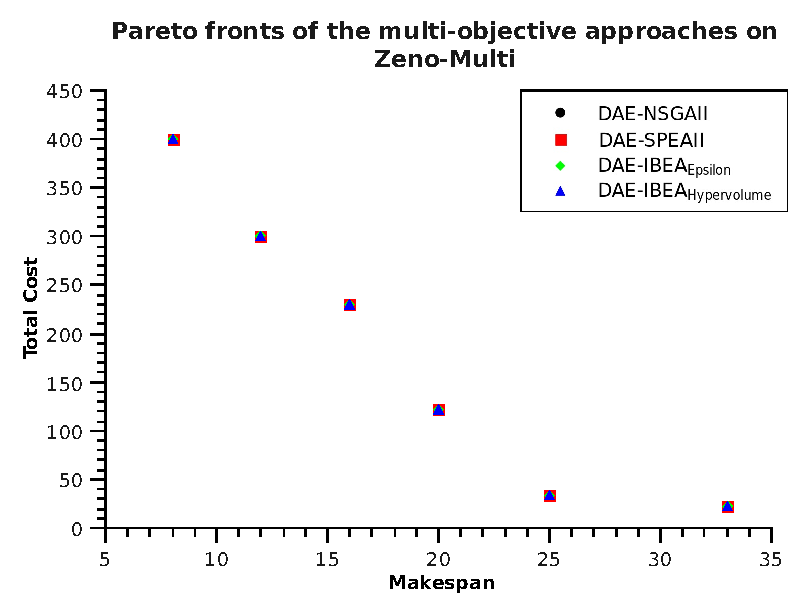
\includegraphics[bb=0 -0.250000 370.750 278.250]{./pareto_zeno_add.eps}
 % paretofronts.eps: 0x0 pixel, 300dpi, 0.00x0.00 cm, bb=0 -0.250000 370.750 278.250
\end{center}
\end{figure}

\begin{center}
 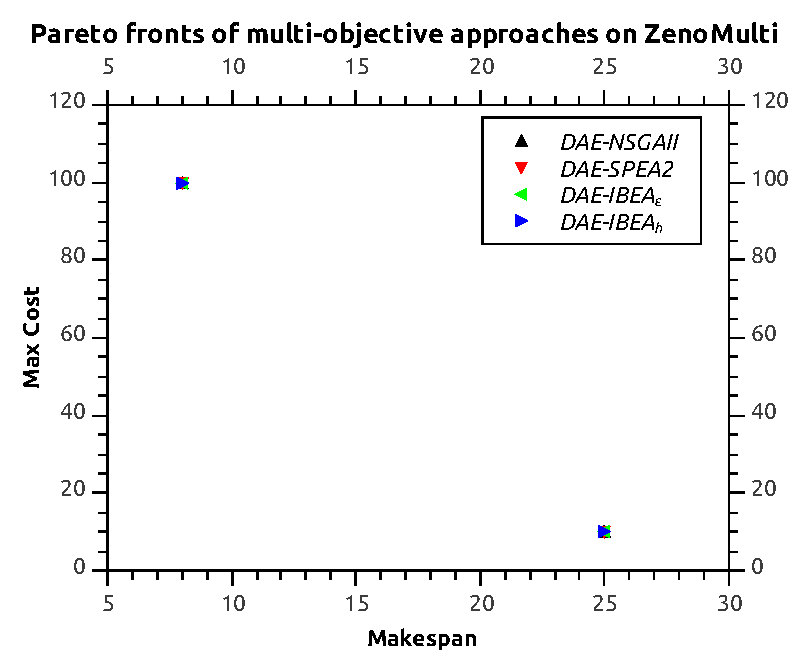
\includegraphics[bb=0 -0.250000 371.500 278.250]{./pareto_zeno_max.eps}
 % daespeaIIzenomax.eps: 0x0 pixel, 300dpi, 0.00x0.00 cm, bb=0 -0.250000 371.500 278.250
\end{center}


\begin{center}
 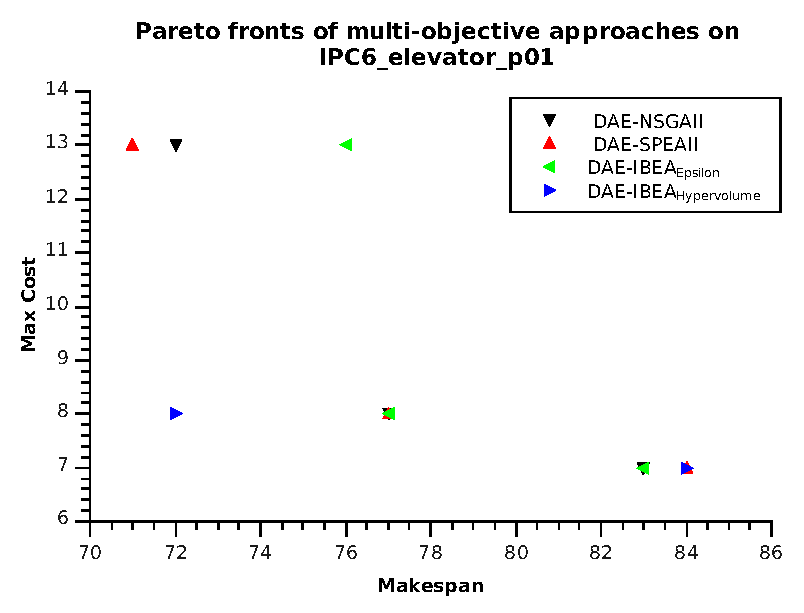
\includegraphics{./pareto_p01_max.eps}
 % paretofronts.eps: 0x0 pixel, 300dpi, 0.00x0.00 cm, bb=0 -0.250000 368.500 278.250
\end{center}
\begin{center}
 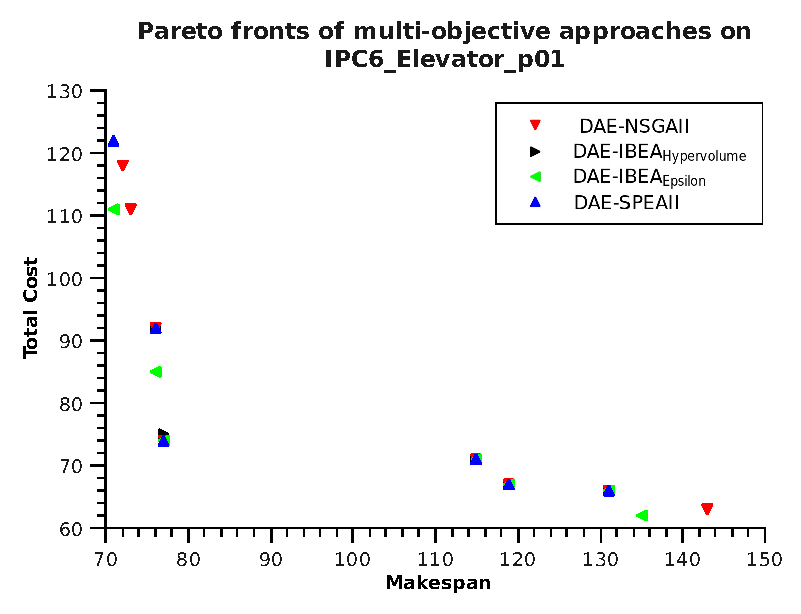
\includegraphics{./pareto_p01_add.eps}
 % paretofronts_max.eps: 0x0 pixel, 300dpi, 0.00x0.00 cm, bb=0 -0.250000 368.500 278.250
\end{center}
\begin{center}
 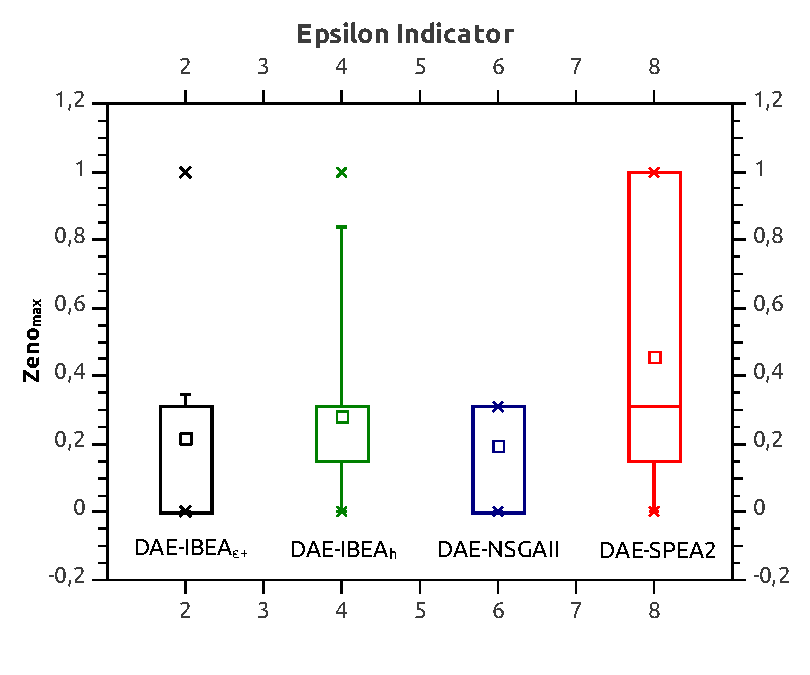
\includegraphics{./bp_zeno_max_eps.eps}
 % bp_zeno_max_eps.eps: 0x0 pixel, 300dpi, 0.00x0.00 cm, bb=0 0 373 308
\end{center}
\begin{center}
 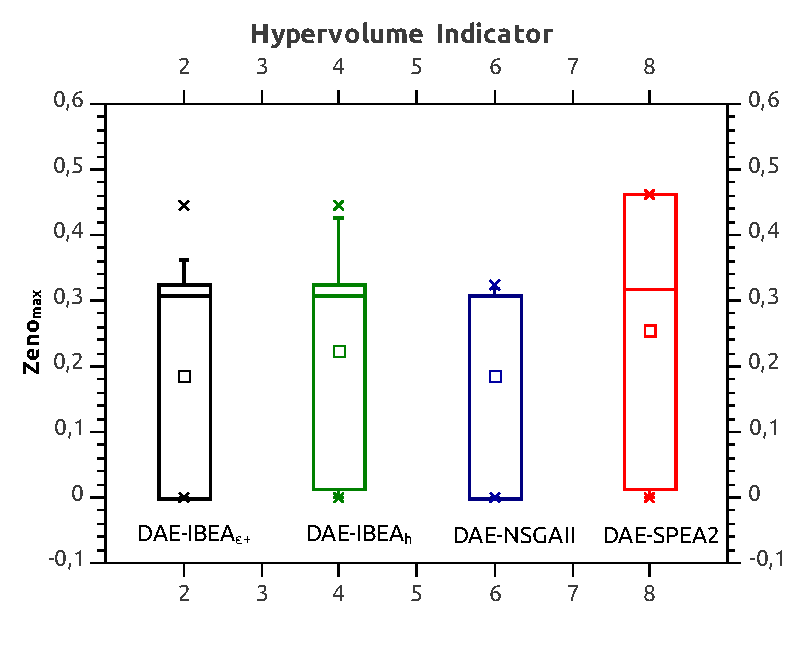
\includegraphics[bb=0 0 370 300]{./bp_zeno_max_hyper.eps}
 % bp_zeno_max_hyper.eps: 0x0 pixel, 300dpi, 0.00x0.00 cm, bb=0 0 370 300
\end{center}

\begin{center}
 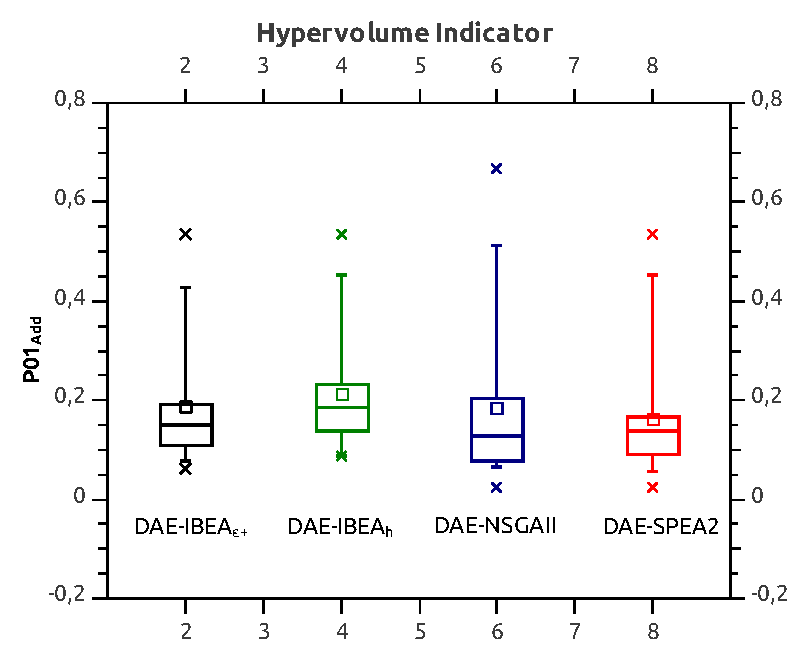
\includegraphics{./bp_p01_add_hyper.eps}
 % bp_p01_add_hyper.eps: 0x0 pixel, 300dpi, 0.00x0.00 cm, bb=0 0 372 303
\end{center}
\begin{center}
 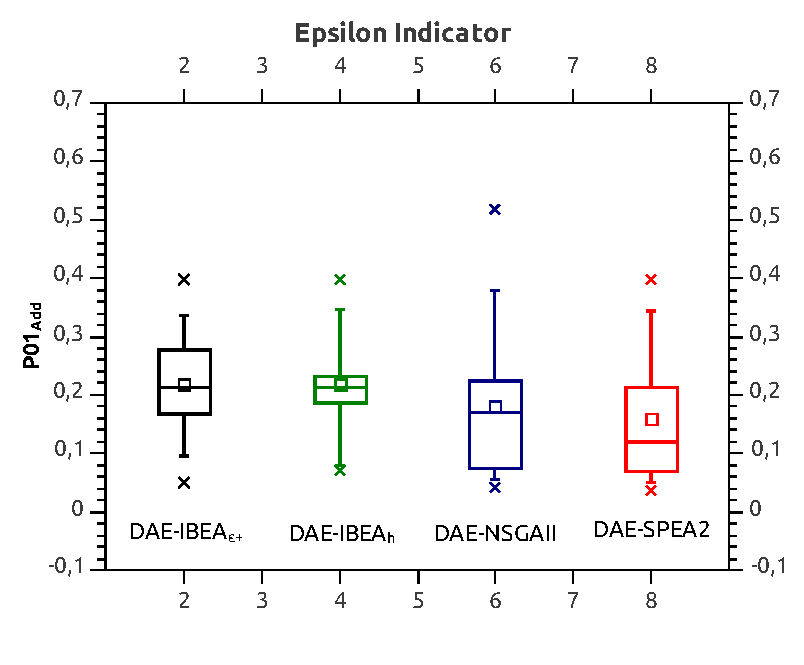
\includegraphics[bb=0 0 370 303]{./bp_p01_Add_eps.eps}
 % bp_p01_Add_eps.eps: 0x0 pixel, 300dpi, 0.00x0.00 cm, bb=0 0 370 303
\end{center}
\begin{center}
 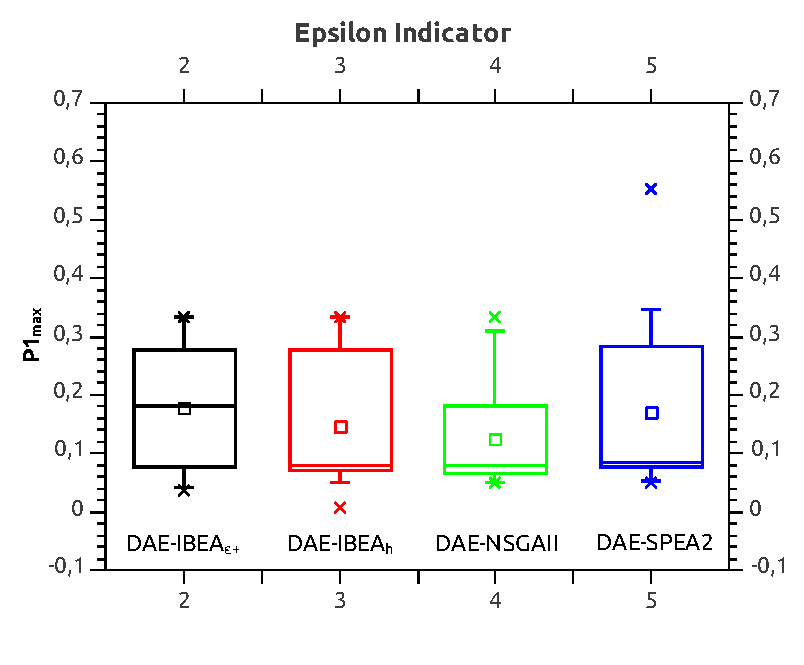
\includegraphics[bb=0 0 370 303]{./bp_p01_Max_eps.eps}
 % bp_p01_Max_eps.eps: 0x0 pixel, 300dpi, 0.00x0.00 cm, bb=0 0 370 303
\end{center}
\begin{center}
 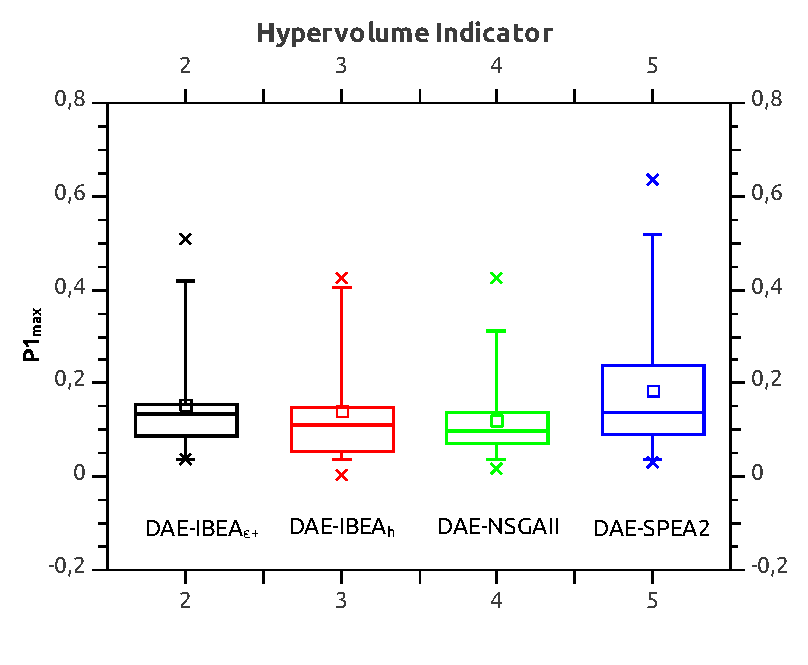
\includegraphics[bb=0 0 372 303]{./bp_p01_Max_hyp.eps}
 % bp_p01_Max_hyp.eps: 0x0 pixel, 300dpi, 0.00x0.00 cm, bb=0 0 372 303
\end{center}

 %\end{landscape}
\end{document}          


